\documentclass[a4paper,12pt]{article}

\usepackage[utf8]{inputenc}
\usepackage[english,ngerman]{babel}
\selectlanguage{ngerman}

\usepackage[T1]{fontenc}
\usepackage{amsmath}
\usepackage{graphicx}
\usepackage{graphviz}

\usepackage{amsfonts}

\usepackage{url}
\usepackage[colorlinks=false,pdfborder={0 0 0},breaklinks=true]{hyperref}


\begin{document}

\title{Konzeptpapier Lichtsteuerung}
\author{Marius \textbf{Schuller}\\
        Stefan \textbf{Thiemann}\\
		Patrick \textbf{Wildt}}
\maketitle

\tableofcontents

\newpage

\noindent
Hier soll kurz die Grundidee des Schwerpunktprojekts, sowie welche Hardware 
benötigt wird, beschrieben werden.

\section{Einführung}

Im Zuge der Internet-of-Things-Kampagne\footnote{\url{http://www.nextgenerationmedia.de}}
werden immer weitere ``dumme'' Geräte miteinander intelligent vernetzt. Dazu
gehören auch Lichter und Glühbirnen. Zur Vernetzung und Steuerung der Lichter
existieren bereits mehrere aktuelle Technologien. Mit Hilfe einer der
standardisierten Technologie möchten wir einen Controller implementieren,
welcher diese Lichter kontrollieren kann.

\section{Lichtsteuerungs-Technologien}

Üblicherweise möchten Hersteller ein eigenes Produkt-Ökosystem erstellen, aus dem die
Anwender kaum mehr ausbrechen können. In Folge dessen werden eigene Protokolle
implementiert. Beispielsweise bietet \textit{LimitlessLED}
\footnote{\url{http://www.limitlessled.com}} Glühbirnen, welche sich
über 2,4 GHz WLAN in das lokale Netzwerk verbinden können. Für die eigentliche
Steuerung wurde eine eigene API entwickelt. Eine weitere bekannte Technologie ist
\textit{Bluetooth}. Hier ist es derzeit möglich mit Hilfe des \textit{Generic
Attribute Profile}, kurz
\textit{GATT}\footnote{\url{https://de.wikipedia.org/wiki/Bluetooth-Profile}},
ein eigenes Protokoll zu sprechen. Dies wird bei mehreren smarten Glühbirnen
verwendet um ein proprietäres Lichtsteuerungsprotokoll zu implementieren.

\newpage

Die \textit{Bluetooth} Konkurrenten
\textit{Z-Wave}\footnote{\url{http://www.z-wavealliance.org}}, welches sich auf das
so genannte \textit{Home Control}-Szenario konzentriert, sowie
\textit{ZigBee}\footnote{\url{http://www.zigbee.org}},
implementieren jeweils eigene Lichtprotokolle. Diese Protokolle sind jedoch für jeden
Client des Funkstandards nutzbar, sodass die Lichterhersteller kein eigenes Protokoll
implementieren müssen. Der Funkstandard \textit{ZigBee} wird von den namhaften
Herstellern \textit{Philips} und \textit{Osram} verwendet.

Für das Schwerpunktprojekt würden wir uns auf \textit{ZigBee} kompatible Geräte
konzentrieren. Vor allem die Produkte der \textit{Philips hue} Reihe.

\section{Komponenten}

Die eigentliche Logik zur Steuerung der Lichter kann auf einem \textit{RaspberryPi}
implementiert werden. Um den Funkstandard \textit{ZigBee} sprechen zu können wird ein
kompatibles Funkmodul benötigt. Hierfür kann das \textit{RaspBee}-Modul verwendet werden.
Dieses gibt es in zwei Varianten, \textit{Basic} und \textit{Premium}. Während man mit der
Basic-Variante nur mit 5 Knoten sprechen darf, ist dies bei der Premium-Variante
unbegrenzt. Die Lichter würden aus einem \textit{Philips Hue} Starterkit bestehen.

\section{Liste}

\subsection{Variante RaspBee Basic}

\begin{tabular}{p{2cm}p{4.5cm}p{3cm}p{3cm}}
   Menge & Produkt & Einzelpreis & Gesamtpreis\\
   \hline
   3 & RaspberryPi 2 & 42 Euro & 126 Euro\\
   3 & RaspBee Basic & 31 Euro & 93 Euro\\
   1 & Philips hue Starterkit \newline 3 x 9W A60 E27 & 169 Euro & 169 Euro\\
   \hline
   Gesamtpreis & & & \textbf{388 Euro}\\
\end{tabular}

\subsection{Variante RaspBee Premium}

\begin{tabular}{p{2cm}p{4.5cm}p{3cm}p{3cm}}
   Menge & Produkt & Einzelpreis & Gesamtpreis\\
   \hline
   3 & RaspberryPi 2 & 42 Euro & 126 Euro\\
   3 & RaspBee Premium & 49 Euro & 147 Euro\\
   1 & Philips hue Starterkit \newline 3 x 9W A60 E27 & 169 Euro & 169 Euro\\
   \hline
   Gesamtpreis & & & \textbf{442 Euro}\\
\end{tabular}

\subsection{Hinweis}

Unter Umständen sind Bestandteile der Liste schon im Vorrat der Hochschule oder
der Projektteilnehmer. Je nach Beteiligung der Fachhochschule würden wir für einen
Teil der Kosten aufkommen.

\section{Grobarchitektur}

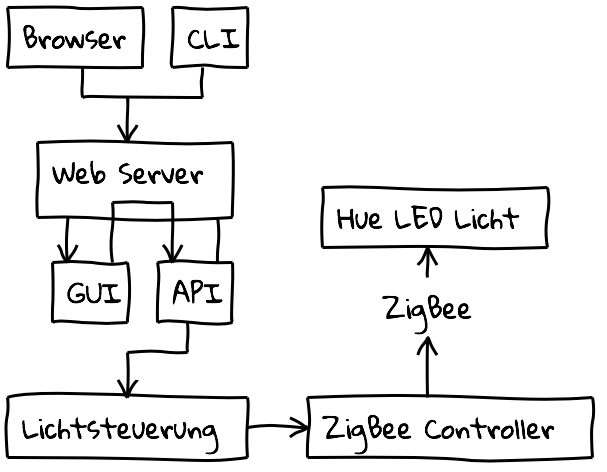
\includegraphics[width=\linewidth]{grobarchitektur}

\end{document}